\documentclass{article}

\title{Design Document for The Flying Dutchman}
\author{Max Block \and Linda Eriksson \and Daniel Llatas Spiers \and Joakim Järvinen \and Christian Törnqvist \and Joel Wiklund\and \\Group Stormrider\\Version 1.0}
\date{February 2015}

\usepackage{natbib}
\usepackage{graphicx}
\usepackage{hyperref}

\begin{document}



\maketitle
\clearpage

\begin{abstract}
  Abstract.
\end{abstract}
\tableofcontents

\subsection*{Changelog}
\addcontentsline{toc}{subsection}{Changelog}
\paragraph{}
\em{}Version 1.0:\em{} Created document.\\ 
\clearpage

\part{Design Overview}
\section{Personas}
\label{sec:label}
\subsection{Bartender}
Caesar is a 21 years old man, who just finished bartending school. This is the first time ever that he is working at The Flying Dutchman. Although he just finished bartending school, he is also doing academic studies so his work at The Flying Dutchman is not full time. His intention is to work at nights and study daytime in order to finance his studies.
\subsection{Professor}
Bengt is a 53 year old man from Sweden. He is a professor in the field of computer science. He is a very social person who spend a lot of his spare time at The Flying Dutchman where he is on the list of so called VIPs, who have some special privileges over other customers. Bengt enjoys drinking beer and especially trying out rare special beers which may not be available in your local liquor store. Socially, he enjoy talking with students at the bar about their life choices and giving them some valuable advice.
\subsection{Student}
Alice is a 23 year old girl who is an international student from USA that loves to be around people. She enjoys going out partying and wants to do it as often as possible. However, as an international student, she has a very limited budget and thus have to think economically when going out. She really likes being in Sweden and plans on learning the language so that she can settle down there.
\subsection{Manager}
Marie is a 35 year old Swedish woman with great experience as a pub manager. During her twenties, she was a student at Uppsala University, however, studying was not the thing that got the most of her attention but rather spending time and working at nations. She worked so much that she had to take a break from her studies. She never got back from her break but she had figured that she wanted to work full time in bars. This resulted in her applying to The Flying Dutchman where she got employed and it did not take long before she became the manager.
\section{Scenarios}
\label{sec:label}
\subsection{Student}
\begin{itemize}
\item Goes to the bar and asks the bartender for the cheapest beer possible. The bartender, who has just started his career, doesn’t know the menu and has to search in the system for the cheapest beer. He finds the beer, bring it and gives it to Alice. Alice pays both by cash and by card.
\item Alice now wants a second round and orders two beers. This time she tries to pay only by card. But she doesn’t have enough money, so the bank rejects the payment. She tells the bartender to remove one beer and tries to pay again. Once again the payment doesn’t go through so the bartender cancels the order.

\end{itemize}
\subsection{Professor}

\begin{itemize}
\item He goes to the VIP terminal, logs in and looks at the available beers. So he picks one of his favorite beers, a nice Belgian Ale. He checks that he has enough credit and then checkouts. After that, he goes and grabs the beer.
\item The professor wants to become a VIP customer. So he goes to the manager and asks to become a VIP. The manager approves and gives Bengt a register code. Bengt goes to the VIP terminal, type in the code and fills in a form with his personal data.
\item The professor has used all his credit. He goes to the bartender to refill his credit. 

\end{itemize}
\subsection{Bartender}

\begin{itemize}
\item A customer comes and wants to know which beers from "Brewdog" are available at the bar. So Caesar searches for "Brewdog", and the system displays a list of these beers. The customer says what he wants, the bartender selects it and goes to checkout.
\item A customer wants a Heineken. Caesar selects Heineken as it is the most common beer and goes to checkout.

\end{itemize}
\subsection{Manager}

\begin{itemize}
\item The system makes a suggestion for the beers to ordered. And then the manager can edit by adding/subtracting numbers, add a new type of or deleting items. He then approves the order.
\item The manager can add a new bartender.
\item The manager can add a new regular.

\end{itemize}
\section{Requirements specification}

\clearpage
\section{Prototype}
\begin{figure}[h!]
\centering
\frame{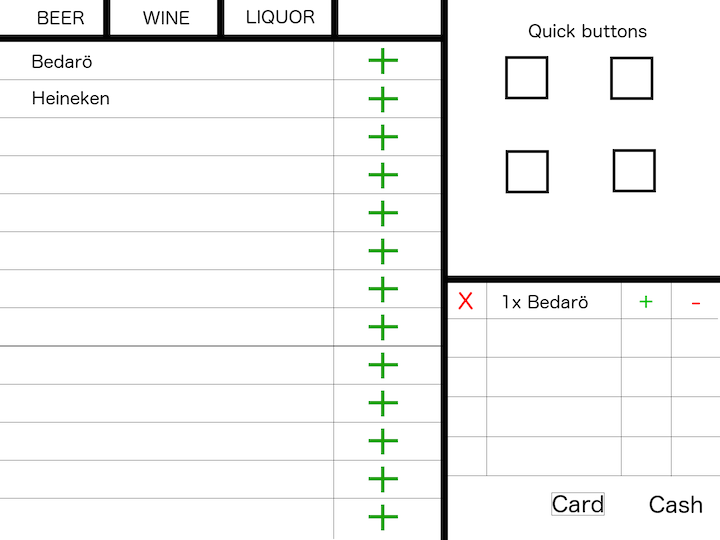
\includegraphics[width=\textwidth, height=\textheight, keepaspectratio, natwidth=720, natheight=540]{mockup_small.png}}
\caption{Prototype mockup}
\label{fig:mockup}
\end{figure}

\clearpage
\section{UML}
\subsection{Cart component}
\begin{figure}[!htb]
\centering
\frame{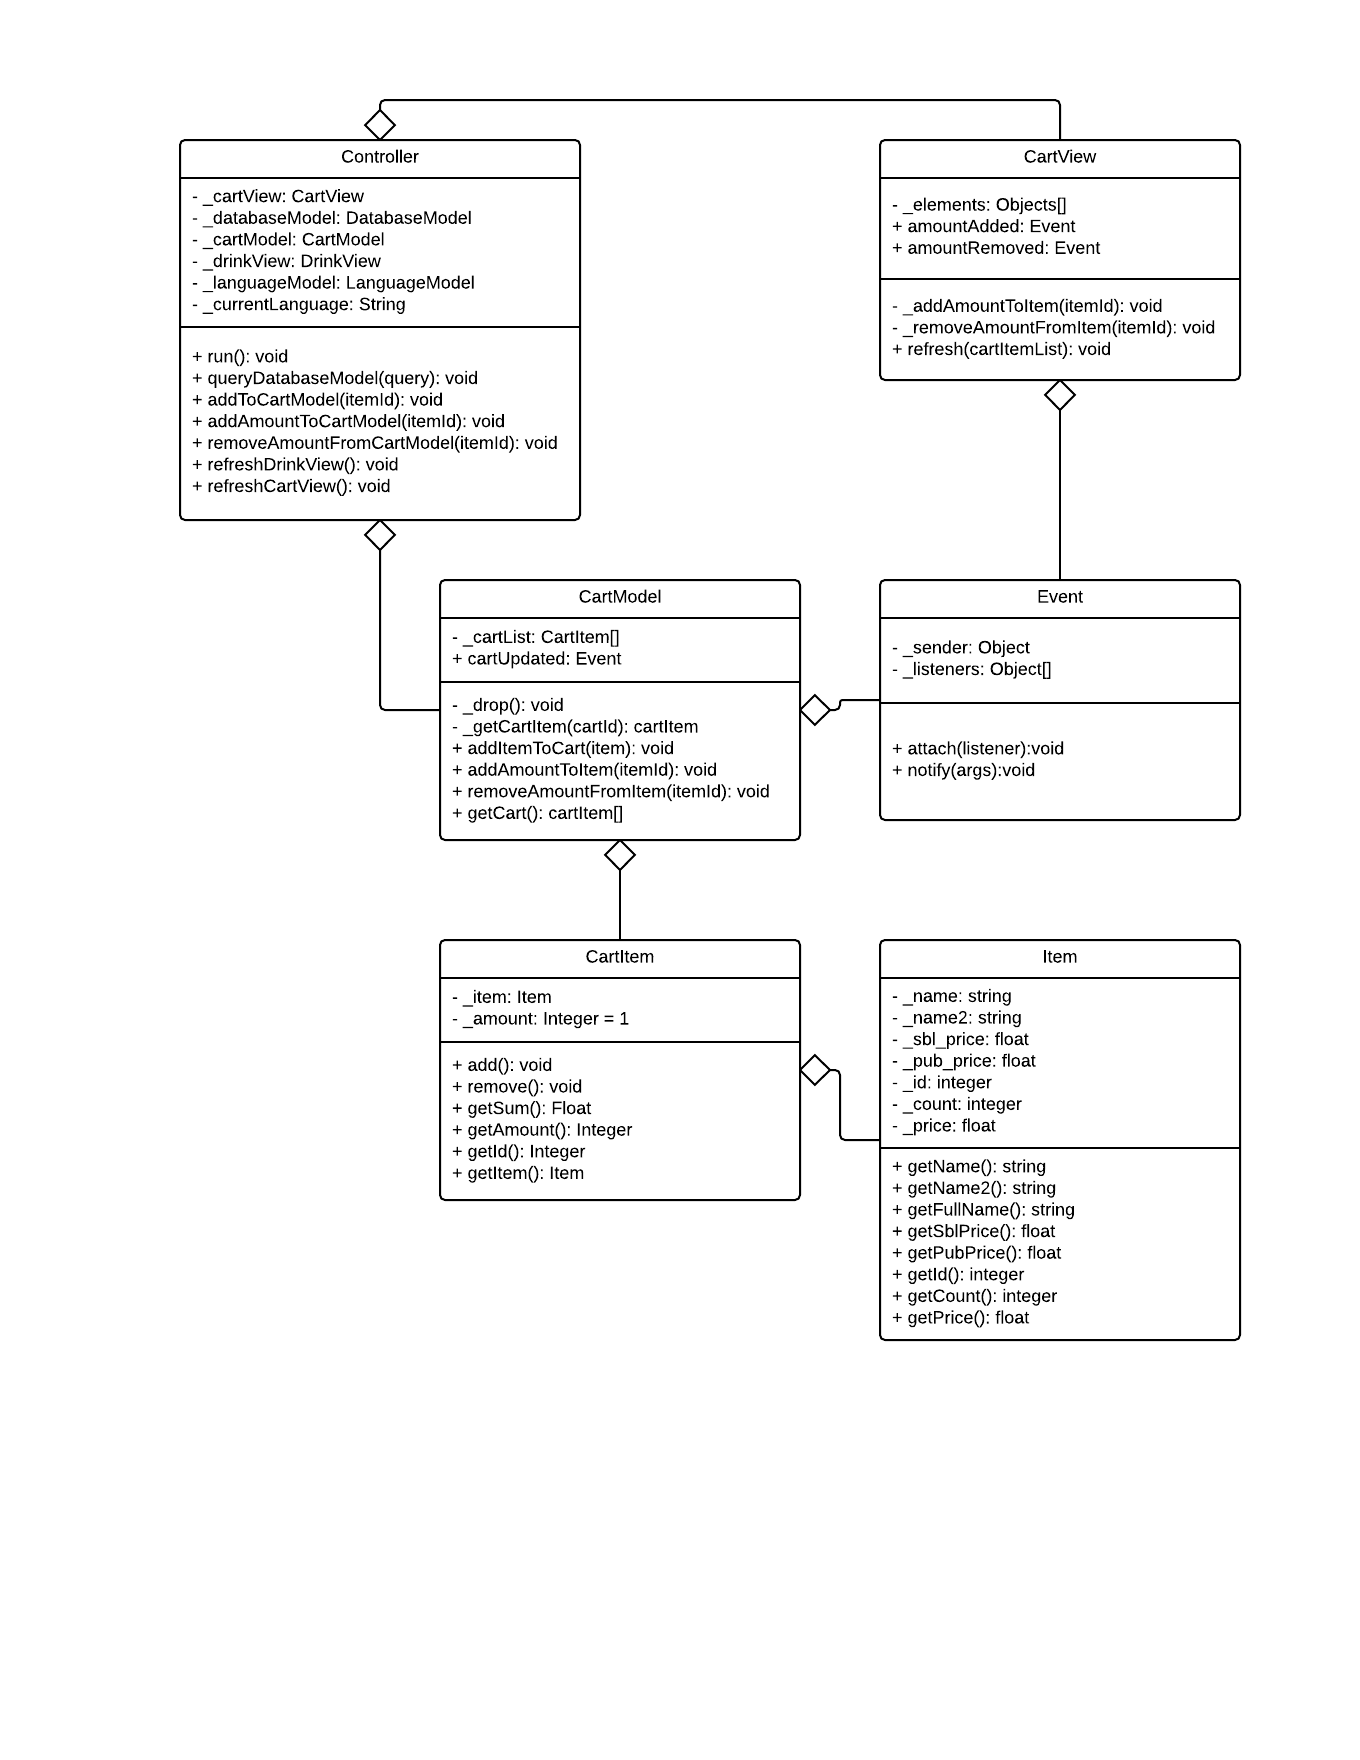
\includegraphics[width=\textwidth, height=\textheight, keepaspectratio, natwidth=1202, natheight=1123]{cartUml.png}}
\caption{Cart UML}
\label{fig:cartUml}
\end{figure}

\clearpage
\subsection{Drink component}
\begin{figure}[!htb]
\centering
\frame{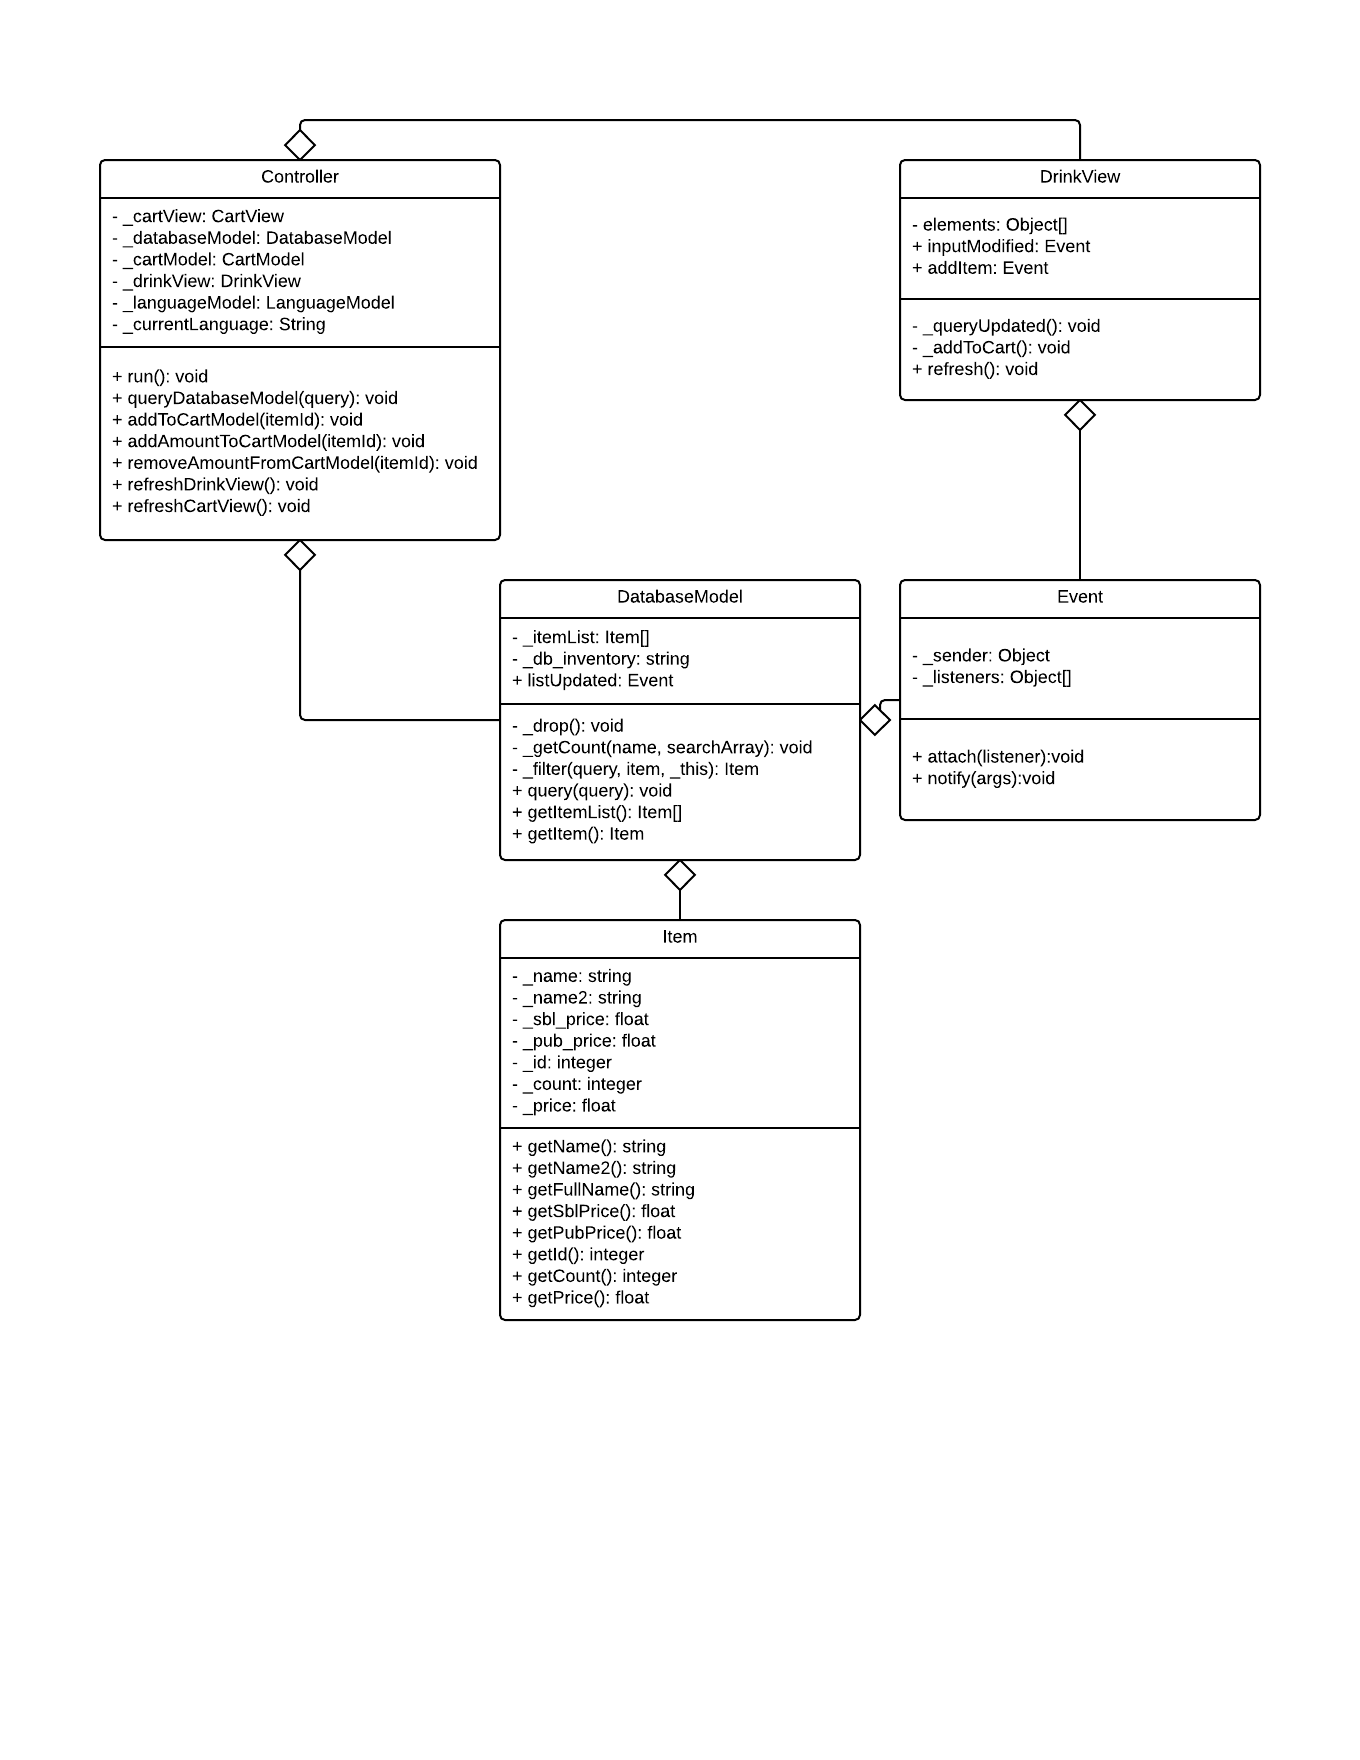
\includegraphics[width=\textwidth, height=\textheight, keepaspectratio, natwidth=1202, natheight=1123]{drinkUml.png}}
\caption{Drink UML}
\label{fig:drinkUml}
\end{figure}

\clearpage
\subsection{Language component}
\begin{figure}[!htb]
\centering
\frame{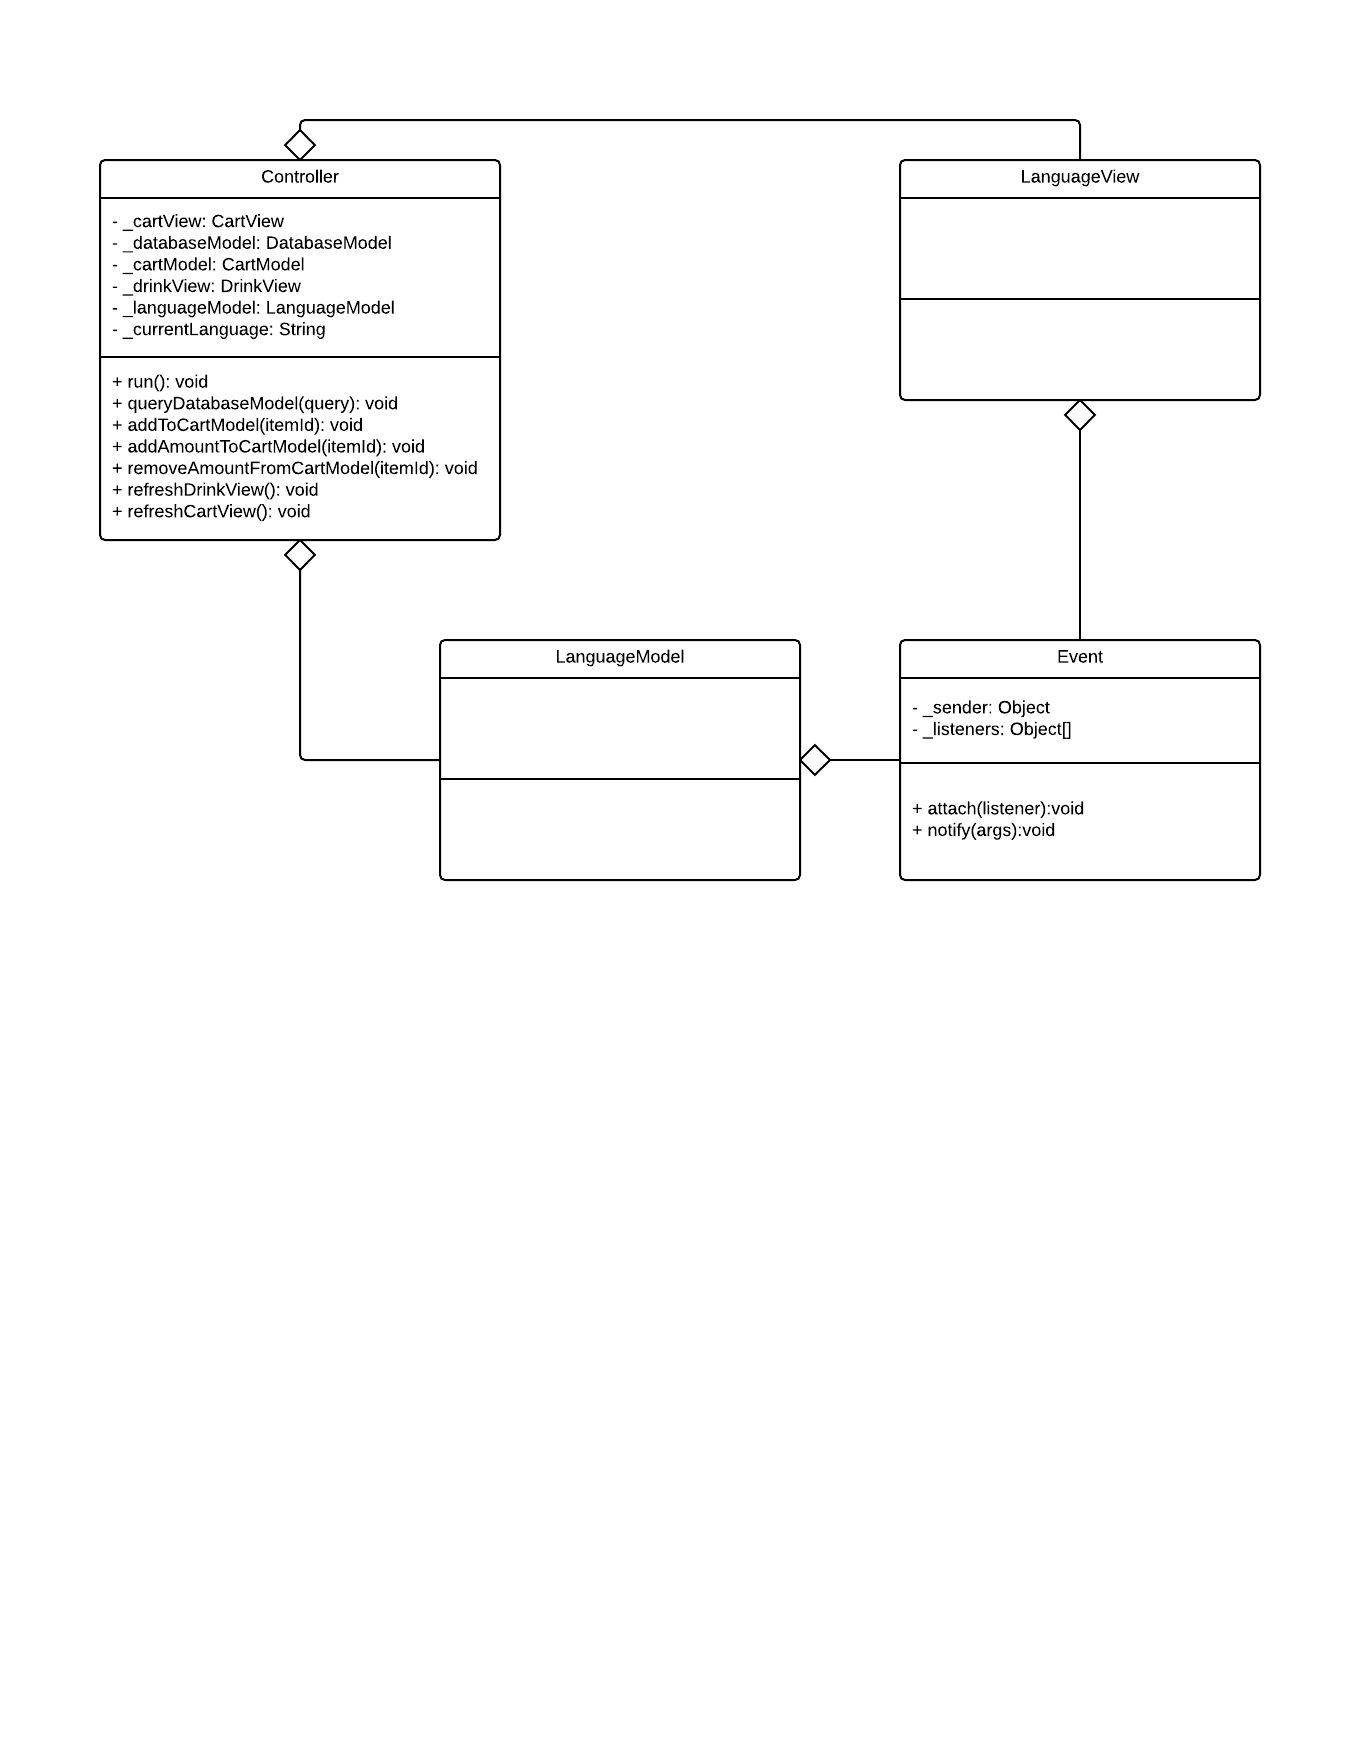
\includegraphics[width=\textwidth, height=\textheight, keepaspectratio, natwidth=1202, natheight=1123]{languageUml.png}}
\caption{Language UML}
\label{fig:languageUml}
\end{figure}

\clearpage
\subsection{Login component}
\begin{figure}[!htb]
\centering
\frame{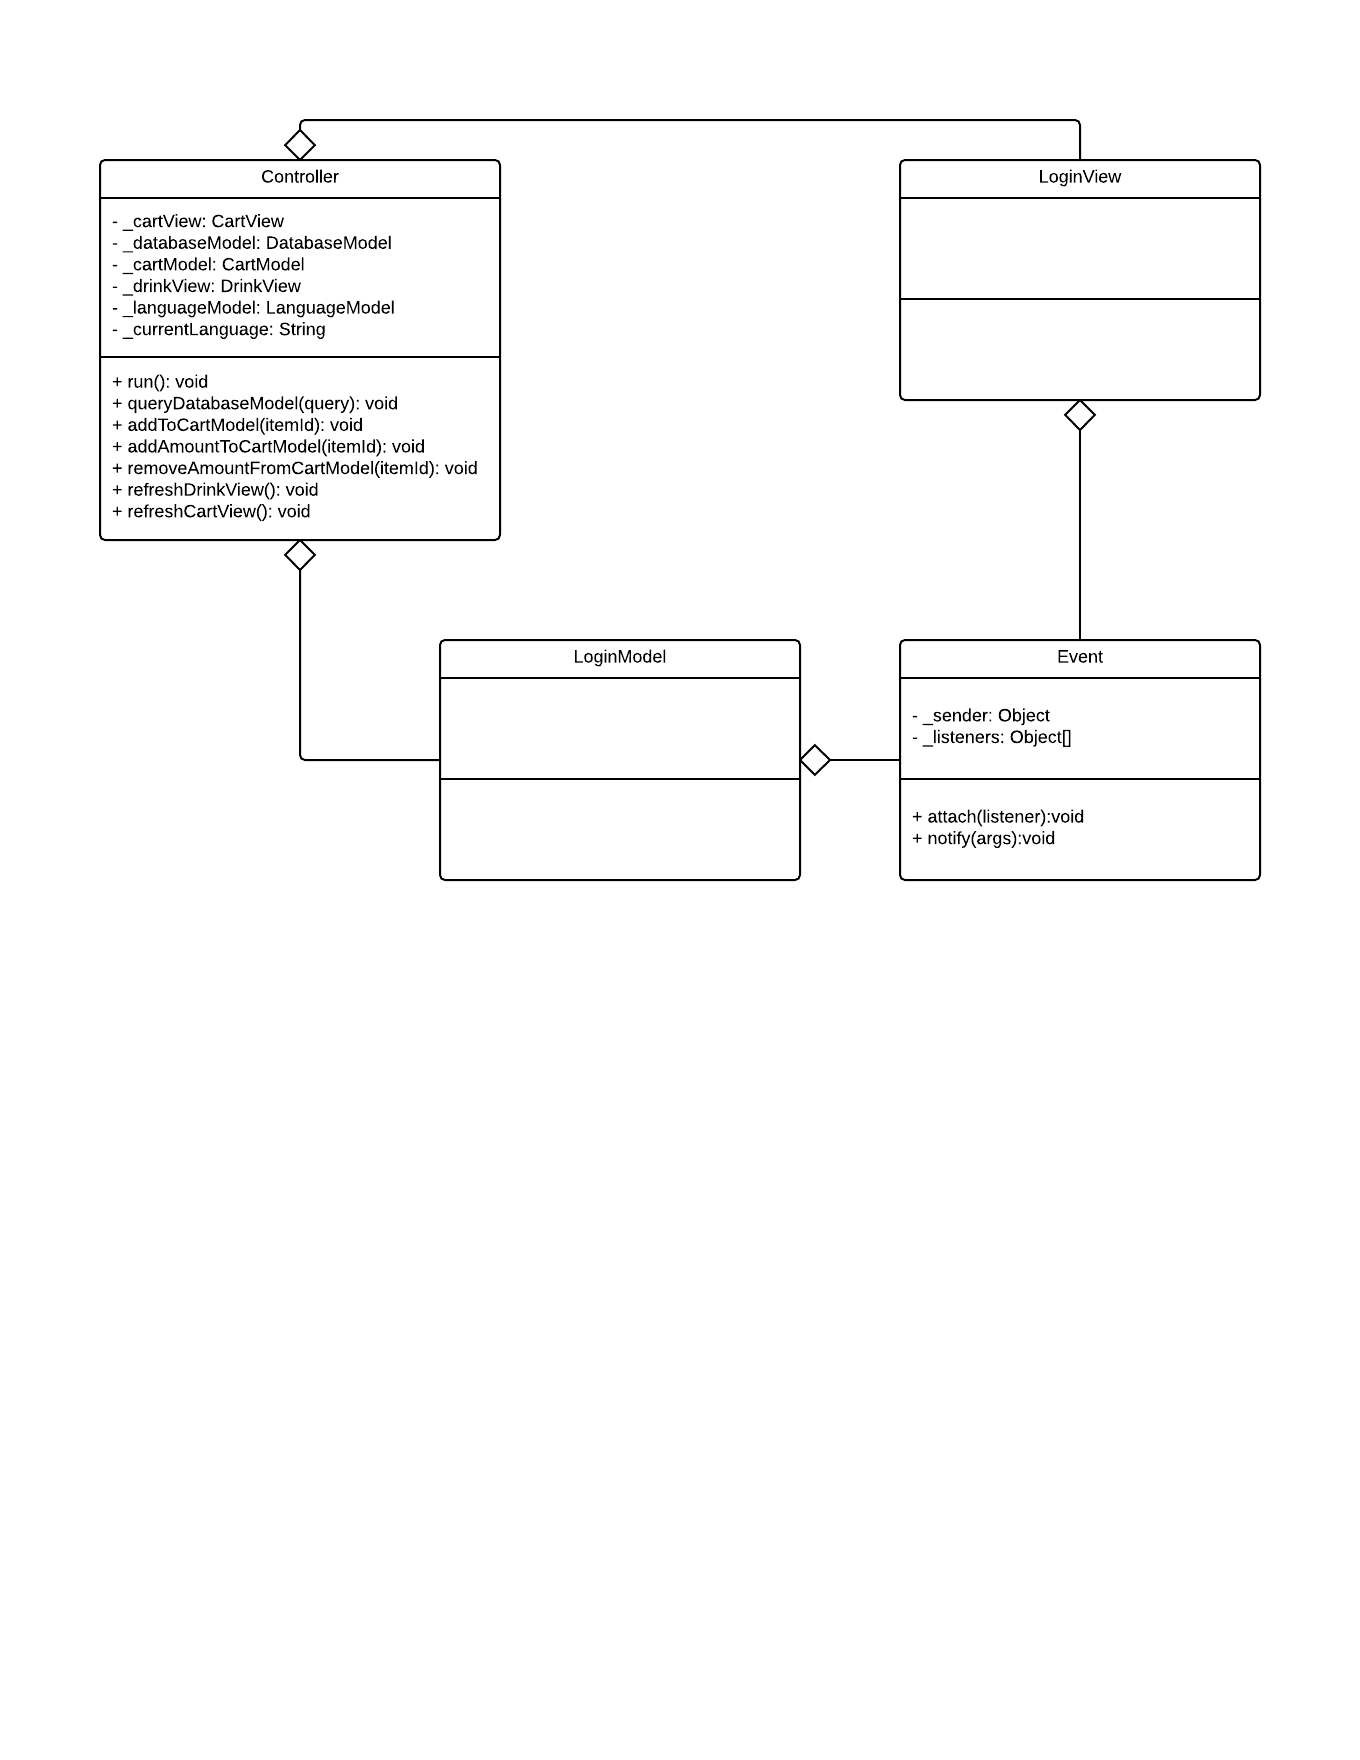
\includegraphics[width=\textwidth, height=\textheight, keepaspectratio, natwidth=1202, natheight=1123]{loginUml.png}}
\caption{Login UML}
\label{fig:loginUml}
\end{figure}

\clearpage
\subsection{Quick component}
\begin{figure}[!htb]
\centering
\frame{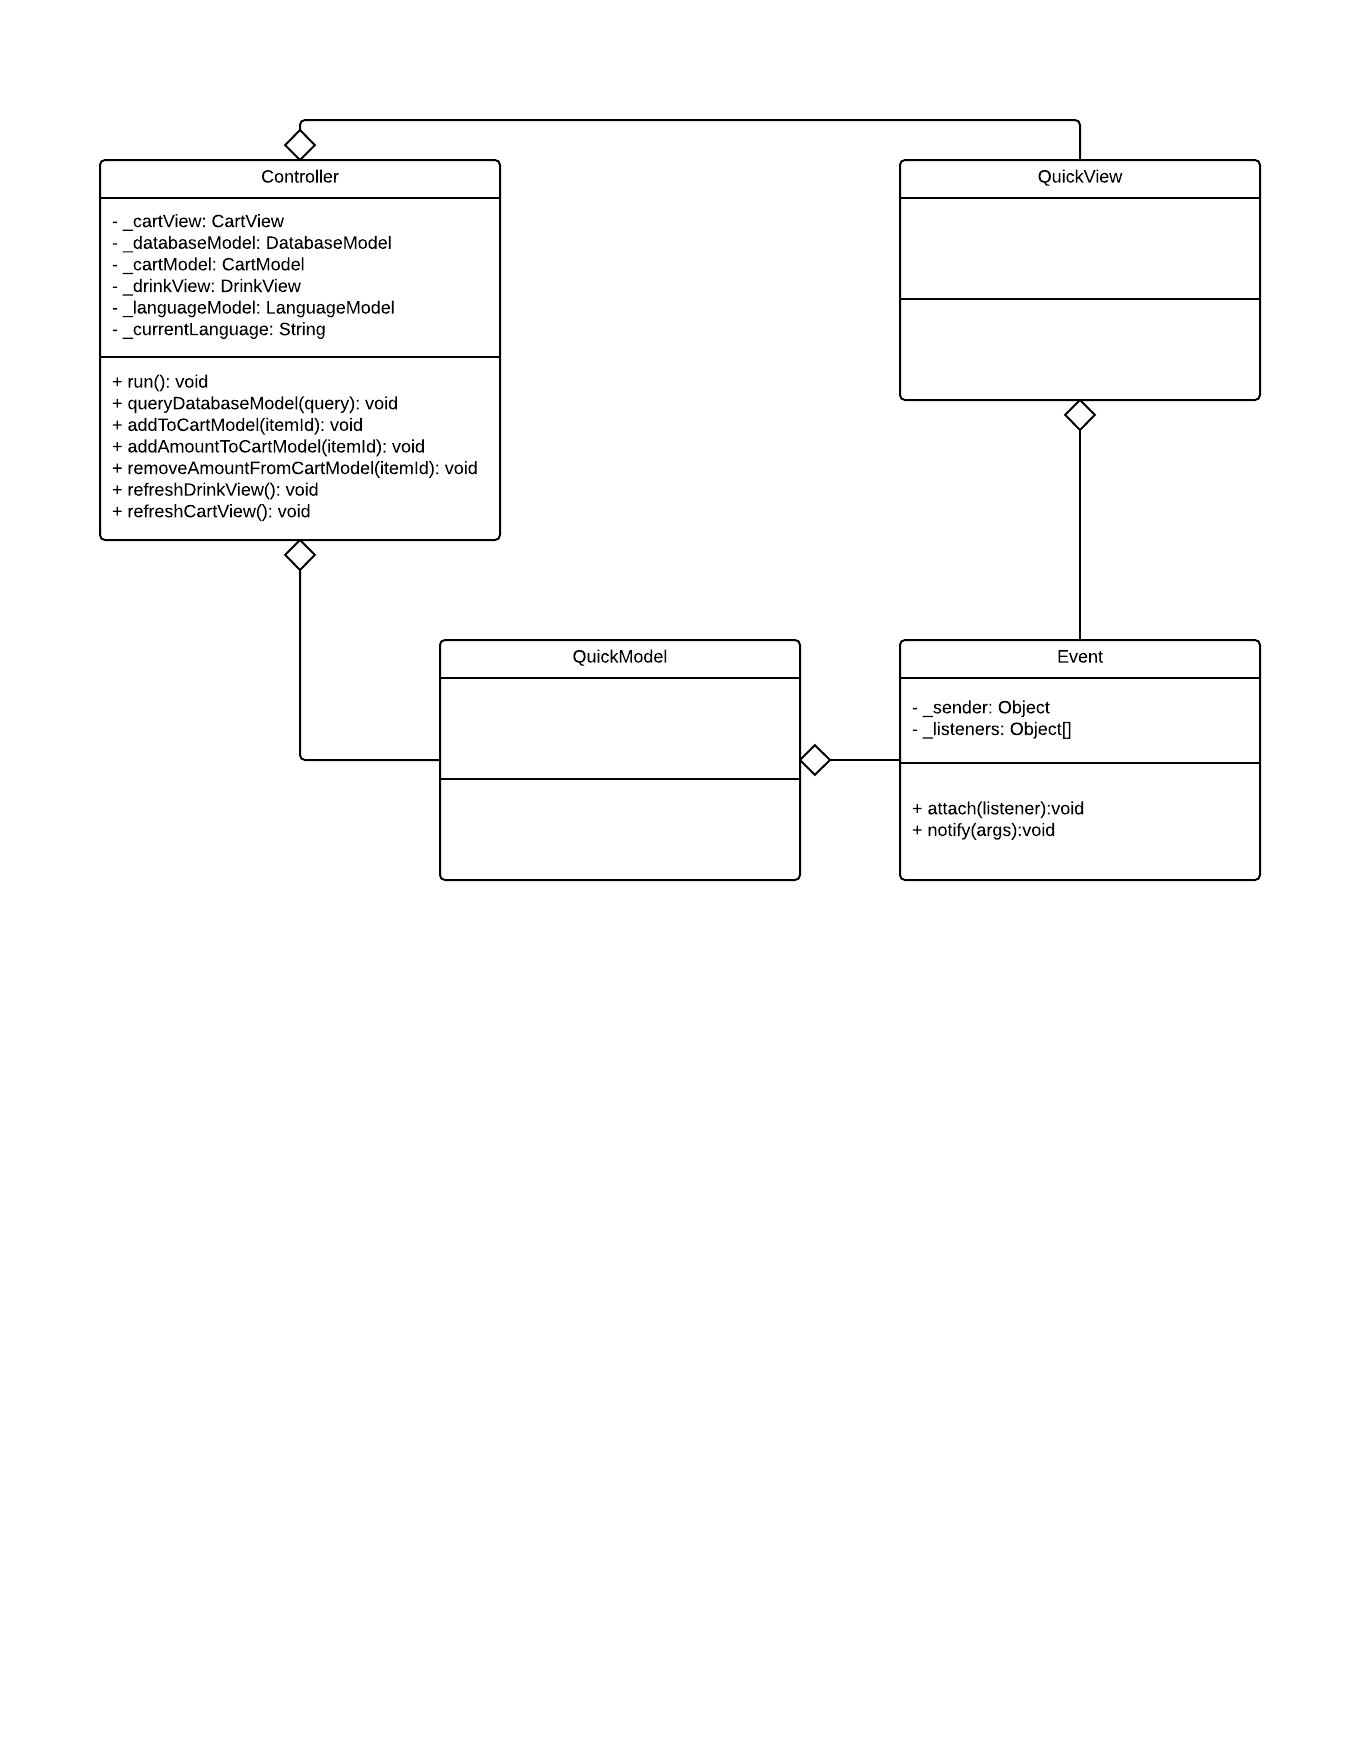
\includegraphics[width=\textwidth, height=\textheight, keepaspectratio, natwidth=1202, natheight=1123]{quickUml.png}}
\caption{Quick UML}
\label{fig:quickUml}
\end{figure}


\clearpage
\section{Database API}
\subsection{admin}
\subsubsection{inventory\_get}
Gives a list of all drinks available in the system.\\
\textbf{Parameters:}\\
none\\
\textbf{Returns:}\\
JSON-object:\\
- type: "inventory\_get"\\
- payload[]\\
\indent - namn\\
\indent - namn2\\
\indent - sbl\_price\\
\indent - pub\_price\\
\indent - beer\_id\\
\indent - count\\
\indent - price\\
\textbf{Usage:}\\
\url{http://pub.jamaica-inn.net/fpdb/api.php?username=ervtod\&password=ervtod\&action=inventory\_get}\\

\subsubsection{purchases\_get\_all}
Gives a list of all purchases made by all users.\\
\textbf{Parameters:}\\
none\\
\textbf{Returns:}\\
JSON-object:\\
- type: "purchases\_get"\\
- payload[]\\
\indent - namn\\
\indent - namn2\\
\indent - transaction\_id\\
\indent - user\_id\\
\indent - beer\_id\\
\indent - timestamp\\
\indent - price\\
\indent - first\_name\\
\indent - last\_name\\
\indent - username\\
\textbf{Usage:}\\
\url{http://pub.jamaica-inn.net/fpdb/api.php?username=ervtod\&password=ervtod\&action=purchases\_get\_all}\\

\subsubsection{payments\_get\_all}
Returns a list of payments made by all users.\\
\textbf{Parameters:}\\
none\\
\textbf{Returns:}\\
JSON-object:\\
- type: "payments\_get\_all"\\
- payload[]\\
\indent - admin\_username\\
\indent - timestamp\\
\indent - amount\\
\indent - admin\_id\\
\indent - username\\
\indent - first\_name\\
\indent - last\_name\\
\textbf{Usage:}\\
\url{http://pub.jamaica-inn.net/fpdb/api.php?username=ervtod\&password=ervtod\&action=payments\_get\_all}\\
 
\subsubsection{iou\_get\_all}
Returns all users and amounts they have at their disposal. For users with a negative balance it means that they have a debt.\\
\textbf{Parameters:}\\
none\\
\textbf{Returns:}\\
JSON-object:\\
- type: "iou\_get\_all"\\
- payload[]\\
\indent - user\_id\\
\indent - first\_name\\
\indent - last\_name\\
\indent - assets\\
\textbf{Usage:}\\
\url{http://pub.jamaica-inn.net/fpdb/api.php?username=ervtod\&password=ervtod\&action=iou\_get\_all}\\
    
\subsubsection{user\_edit}
Updates user information. All user information is required as additional parameters.\\
\textbf{Parameters:}\\
new\_username\\
new\_password\\
first\_name\\
last\_name\\
email\\
phone\\
\textbf{Returns:}\\
JSON-object:\\
- type: "User user added"\\
- payload[]\\
\textbf{Usage:}\\
\url{http://pub.jamaica-inn.net/fpdb/api.php?username=ervtod\&password=ervtod\&action=user\_edit\&new\_username=newusername\&new\_password=newpassword\&first\_name=firstname\&last\_name=lastname\&email=email\&phone=phone}\\
 
\subsubsection{inventory\_append}
Updates the number of bottles available in stock and the price for a particular beer. The id of the beer to be updated is required along with its price and current amount of available bottles.\\
\textbf{Parameters:}\\
beer\_id\\
amount\\
price\\
\textbf{Returns:}\\
JSON-object:\\
- type: "empty"\\
- payload[]\\
\textbf{Usage:}\\
\url{http://pub.jamaica-inn.net/fpdb/api.php?username=ervtod\&password=ervtod\&action=inventory\_append\&amount=amount\&price=price}\\

\subsection{user}
\subsubsection{purchases\_get}
Gives a list of all purchases made by the specified user.\\
\textbf{Parameters:}\\
none\\
\textbf{Returns:}\\
JSON-object:\\
- type: "purchases\_get"\\
- payload[]\\
\indent  - namn\\
\indent  - namn2\\
\indent  - transaction\_id\\
\indent  - user\_id\\
\indent  - beer\_id\\
\indent  - timestamp\\
\indent  - price\\
\textbf{Usage:}\\
\url{http://pub.jamaica-inn.net/fpdb/api.php?username=aamsta\&password=aamsta\&action=purchases\_get}\\
    
\subsubsection{purchases\_append}
Adds a purchase of one beer to the system for the specified user. The id of the beer purchased beer is a required additional parameter.\\
\textbf{Parameters:}\\
beer\_id\\
\textbf{Returns:}\\
JSON-object:\\
- type: empty\\
- payload[]\\
\textbf{Usage:}\\
\url{http://pub.jamaica-inn.net/fpdb/api.php?username=aamsta\&password=aamsta\&action=purchases\_append\&beer\_id=beerid}\\
  
\subsubsection{payments\_get}
Returns a list of payments made by the specified user.\\
\textbf{Parameters:}\\
none\\
\textbf{Returns:}\\
JSON-object:\\
- type: "payments\_get\_all"\\
- payload[]\\
\indent - transaction\_id\\
\indent - user\_id\\
\indent - admin\_id\\
\indent - amount\\
\indent - timestamp\\
\textbf{Usage:}\\
\url{http://pub.jamaica-inn.net/fpdb/api.php?username=aamsta\&password=aamsta\&action=payments\_get}\\

\subsubsection{payments\_append}
Adds a payment of specified amount to the system for the specified user. The amount is a required additional parameter.\\
\textbf{Parameters:}\\
amount\\
\textbf{Returns:}\\
JSON-object:\\
N/A\\
\textbf{Usage:}\\
\url{http://pub.jamaica-inn.net/fpdb/api.php?username=aamsta\&password=aamsta\&action=payments\_append\&amount=amount}\\

\subsubsection{iou\_get}
Returns the total amount that the specified user has at his disposal for buying beer. A negative balance means that the user has a debt.\\
\textbf{Parameters:}\\
none\\
\textbf{Returns:}\\
JSON-object:\\
- type: "iou\_get"\\
- payload[]\\
\indent - user\_id\\
\indent - first\_name\\
\indent - last\_name\\
\indent - assets\\
\textbf{Usage:}\\
\url{http://pub.jamaica-inn.net/fpdb/api.php?username=aamsta\&password=aamsta\&action=iou\_get}\\
 
\subsubsection{beer\_data\_get}
Returns all information available in the system for a specified beer. This includes name, price, alcohol volume, etc. The id of the beer for inquiry is a required additional parameter.\\
\textbf{Parameters:}\\
beer\_id\\
\textbf{Returns:}\\
JSON-object:\\
- type: "beer\_data\_get"\\
- payload[]\\
\indent - nr\\
\indent - artikelid\\
\indent - varnummer\\
\indent - namn\\
\indent - namn2\\
\indent - prisinklmoms\\
\indent - volymiml\\
\indent - prisperliter\\
\indent - saljstart\\
\indent - slutlev\\
\indent - varugrupp\\
\indent - forpackning\\
\indent - forslutning\\
\indent - ursprung\\
\indent - ursprungslandnamn\\
\indent - producent\\
\indent - leverantor\\
\indent - argang\\
\indent - provadargang\\
\indent - alkoholhalt\\
\indent - modul\\
\indent - sortiment\\
\indent - ekologisk\\
\indent - koscher\\
\textbf{Usage:}\\
\url{http://pub.jamaica-inn.net/fpdb/api.php?username=aamsta\&password=aamsta\&action=beer\_data\_get\&beer\_id=beerid}\\



\part{Implementation}

\end{document}
